% Shared style for all Git & GitHub lectures (same look as the N-body course)
\documentclass[11pt,a4paper]{article}
\usepackage[margin=2.3cm]{geometry}
\usepackage[T1]{fontenc}
\usepackage{lmodern}
\usepackage{upquote}   % straight quotes in monospaced text, so commands can be copied
\usepackage{microtype}
% keep '--' as two real hyphens in monospace text (commands like --version)
\DisableLigatures[-,<,>]{family=tt*}
\usepackage{booktabs,enumitem,graphicx,xcolor}
\usepackage{array}
\usepackage{needspace}
\usepackage{longtable}
\usepackage{float}
\usepackage{tikz}
\usetikzlibrary{arrows.meta,calc,positioning,decorations.pathreplacing,shapes.geometric,fit,backgrounds}
\usepackage[most]{tcolorbox}
\usepackage{listings}
\usepackage{fancyhdr}
\usepackage[colorlinks=true,linkcolor=blue!50!black,urlcolor=blue!50!black,citecolor=blue!50!black]{hyperref}

\setlength{\parindent}{0pt}
\setlength{\parskip}{0.6em}
\setlength{\abovecaptionskip}{4pt}
\usepackage[font=small,labelfont=bf]{caption}
\setlist{itemsep=0.2em,topsep=0.3em}

% ---------- colours ----------
\definecolor{cbg}{HTML}{F6F8FA}
\definecolor{ckw}{HTML}{0B5CAD}
\definecolor{ccm}{HTML}{6A737D}
\definecolor{cst}{HTML}{B5451B}
\definecolor{cpart}{HTML}{1F6FB2}
\definecolor{cheavy}{HTML}{C0392B}
\definecolor{cgreen}{HTML}{2E8B57}

% ---------- terminal listings ----------
% In a terminal session, lines starting with "$" are what YOU type.
% Everything else is what Git prints back.
\lstdefinestyle{term}{
  basicstyle=\ttfamily\small, backgroundcolor=\color{cbg},
  frame=single, rulecolor=\color{black!15}, showstringspaces=false,
  breaklines=true, columns=fullflexible, keepspaces=true,
  aboveskip=0.6em, belowskip=0.6em, xleftmargin=4pt, xrightmargin=4pt,
  literate={\$\ }{{\textcolor{cgreen}{\$\ }}}2,
  upquote=true
}
\lstset{style=term}
\newcommand{\code}[1]{\texttt{\small #1}}

% ---------- boxes ----------
\newtcolorbox{history}{colback=yellow!8,colframe=orange!60!black,
  title={History},fonttitle=\bfseries\small,left=4pt,right=4pt,top=2pt,bottom=2pt}
\newtcolorbox{quickfact}{colback=purple!4,colframe=purple!55!black,
  title={Quick fact},fonttitle=\bfseries\small,left=4pt,right=4pt,top=2pt,bottom=2pt}
\newtcolorbox{keyidea}{colback=blue!4,colframe=blue!50!black,
  title={Key idea},fonttitle=\bfseries\small,left=4pt,right=4pt,top=2pt,bottom=2pt}
\newtcolorbox{pitfall}{colback=red!4,colframe=red!55!black,
  title={Pitfall},fonttitle=\bfseries\small,left=4pt,right=4pt,top=2pt,bottom=2pt}
\newtcolorbox{tryit}{colback=teal!5,colframe=teal!55!black,
  title={Try it},fonttitle=\bfseries\small,left=4pt,right=4pt,top=2pt,bottom=2pt,breakable}
\newtcolorbox{homework}[1]{colback=green!4,colframe=green!40!black,
  title={Homework #1},fonttitle=\bfseries\small,left=4pt,right=4pt,top=2pt,bottom=2pt,
  breakable}
\newtcolorbox{goals}{colback=gray!6,colframe=gray!60!black,
  title={Learning goals},fonttitle=\bfseries\small,left=4pt,right=4pt,top=2pt,bottom=2pt}

% Solutions always start on a fresh page, behind a clear warning.
\newcommand{\solutionspage}{%
  \clearpage
  \begin{tcolorbox}[colback=red!6,colframe=red!60!black,halign=center]
    {\Large\bfseries Solutions}\\[0.3em]
    {\small Stop here if you have not tried the homework yet.\\
    Attempt every task first, run the checker, and only then read on.}
  \end{tcolorbox}
}

% ---------- Git diagram styles (TikZ) ----------
\tikzset{
  commit/.style={circle,draw=black!70,fill=blue!10,minimum size=7mm,inner sep=0pt,font=\scriptsize\ttfamily},
  newcommit/.style={commit,fill=orange!25,dashed},
  tag/.style={draw,rounded corners=2pt,font=\scriptsize\ttfamily,inner sep=2pt},
  branchtag/.style={tag,fill=green!15,draw=green!40!black},
  headtag/.style={tag,fill=yellow!30,draw=orange!70!black},
  remotetag/.style={tag,fill=purple!10,draw=purple!60!black},
  area/.style={draw,rounded corners,minimum height=11mm,minimum width=33mm,align=center,font=\small},
  cmdarrow/.style={->,thick,>=Stealth},
  link/.style={->,thick,>=Stealth,black!70},
}

% ---------- header ----------
\pagestyle{fancy}
\fancyhf{}
\renewcommand{\headrulewidth}{0.3pt}
\fancyfoot[C]{\thepage}
\newcommand{\lecturetitle}[3]{%
  \fancyhead[L]{\small\textit{Git \& GitHub from Zero}}
  \fancyhead[R]{\small Lecture #1}
  \begin{center}
    {\Large\bfseries Lecture #1}\\[0.4em]
    {\LARGE\bfseries #2}\\[0.4em]
    {\small #3}
  \end{center}
  \vspace{0.5em}
}

\begin{document}
\lecturetitle{2}{Snapshots: \texttt{add}, \texttt{commit}, and the Three Areas}{Saving versions of your project, the staging area, good messages, and ignoring files}

\begin{goals}
\begin{itemize}
  \item Explain what a \emph{commit} is: a saved snapshot of the whole project.
  \item Name the three areas (working directory, staging area, repository) and what moves files between them.
  \item Use \code{git add} and \code{git commit} to save versions, and read \code{git status} at each step.
  \item Choose which changes go into a commit, and write a clear commit message.
  \item Tell Git to ignore files with \code{.gitignore}, and know why secrets must never be committed.
\end{itemize}
\end{goals}

\section{What is a commit?}

In Lecture 1 you created a repository, but it still has \emph{no history}: \code{git status} said \code{No commits yet}. History is made of \textbf{commits}. A commit is a saved snapshot of your whole project at one moment, together with a message saying what you did, who did it, and when.

A good picture is a save point in a video game. You can keep playing and, if something goes wrong, return to an earlier save point. Unlike a game, you decide when to make a save point and you can name each one.

\begin{figure}[H]
\centering
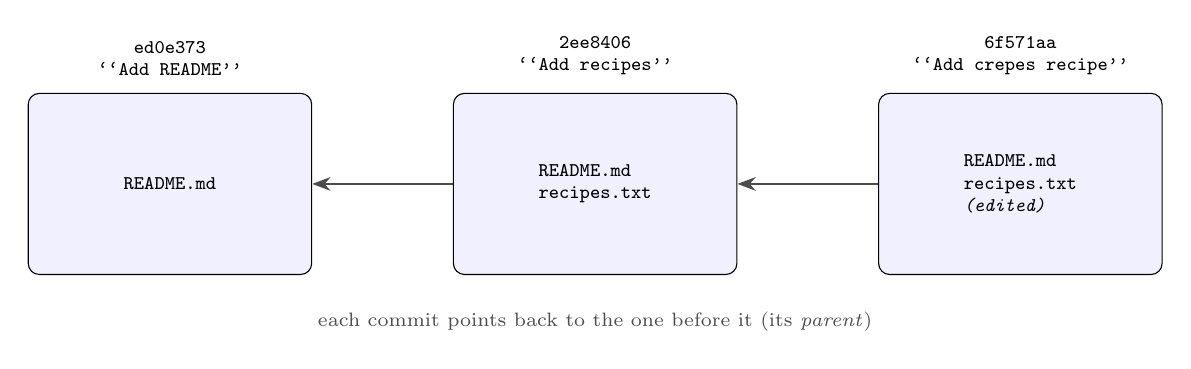
\begin{tikzpicture}[
  snap/.style={draw,rounded corners,fill=blue!6,minimum width=3.6cm,minimum height=2.3cm,align=left,font=\scriptsize\ttfamily,inner sep=6pt},
  idl/.style={font=\scriptsize\ttfamily,align=center}]
  \node[snap] (a) at (0,0)   {README.md};
  \node[snap] (b) at (5.4,0) {README.md\\recipes.txt};
  \node[snap] (c) at (10.8,0) {README.md\\recipes.txt\\\textit{(edited)}};
  \node[idl,above=1mm of a] {ed0e373\\``Add README''};
  \node[idl,above=1mm of b] {2ee8406\\``Add recipes''};
  \node[idl,above=1mm of c] {6f571aa\\``Add crepes recipe''};
  \draw[link] (b.west) -- (a.east);
  \draw[link] (c.west) -- (b.east);
  \node[font=\scriptsize,text=black!70] at (5.4,-1.75) {each commit points back to the one before it (its \emph{parent})};
\end{tikzpicture}
\caption{A history of three commits. Each box is the state of the whole project saved by that commit. The 7-character code is the commit's ID (yours will differ).}
\label{fig:chain}
\end{figure}

\begin{keyidea}
A commit is a \emph{snapshot} of the whole project, not just a list of what changed. (Git is clever about storage: a file that did not change is not copied again.) You can go back to any commit and see the project exactly as it was then.
\end{keyidea}

\begin{quickfact}
Every commit has a unique ID, a 40-character code such as \code{ed0e373a\dots}. Git usually shows just the first 7 characters. The ID is computed from the commit's contents, so in practice no two commits share one.
\end{quickfact}

\section{The three areas}

To make a commit you do not simply ``save''. Git uses \emph{three areas}, and understanding them is the most important idea of the whole course.

\begin{figure}[H]
\centering
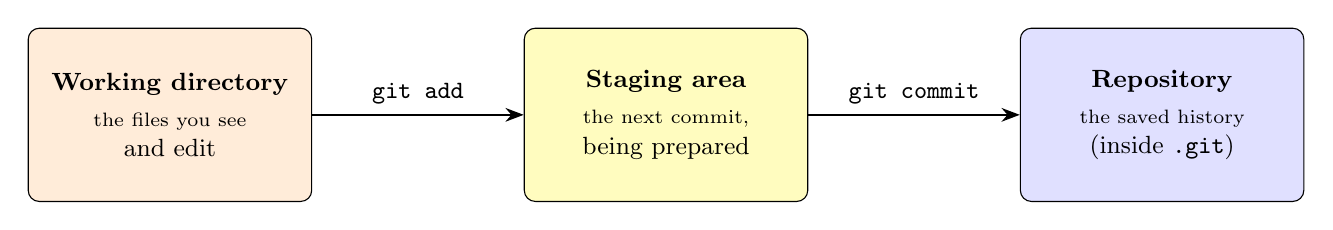
\begin{tikzpicture}[node distance=2.2cm]
  \node[area,fill=orange!15,minimum width=36mm,minimum height=22mm] (wd) at (0,0) {\textbf{Working directory}\\[2pt]\scriptsize the files you see\\and edit};
  \node[area,fill=yellow!25,minimum width=36mm,minimum height=22mm] (st) at (6.3,0) {\textbf{Staging area}\\[2pt]\scriptsize the next commit,\\being prepared};
  \node[area,fill=blue!12,minimum width=36mm,minimum height=22mm] (re) at (12.6,0) {\textbf{Repository}\\[2pt]\scriptsize the saved history\\(inside \code{.git})};
  \draw[cmdarrow] (wd.east) -- node[above,font=\small\ttfamily] {git add} (st.west);
  \draw[cmdarrow] (st.east) -- node[above,font=\small\ttfamily] {git commit} (re.west);
\end{tikzpicture}
\caption{The three areas. Changes move from left to right: first you \emph{stage} the changes you want, then you \emph{commit} what is staged.}
\label{fig:areas}
\end{figure}

\begin{description}[leftmargin=1.2em,style=nextline]
\item[Working directory] The project folder as you see it: the files you create and edit.
\item[Staging area] A waiting room for the next commit. You put in it exactly the changes you want to save together. (Git's own name for it is the \emph{index}.)
\item[Repository] The repository's saved history: all commits, kept in the hidden \code{.git} folder.
\end{description}

Why the extra step? Imagine you fixed a typo in one file and also started a half-finished feature in another. The staging area lets you commit \emph{only the typo fix} now, and the feature later, as separate, meaningful commits.

\begin{quickfact}
The staging area is one of Git's distinctive ideas. Several other version-control tools save all changed files at once, with no step in between.
\end{quickfact}

\subsection{The life of a file}

At any moment, each file in your project is in one of four states:

\begin{figure}[H]
\centering
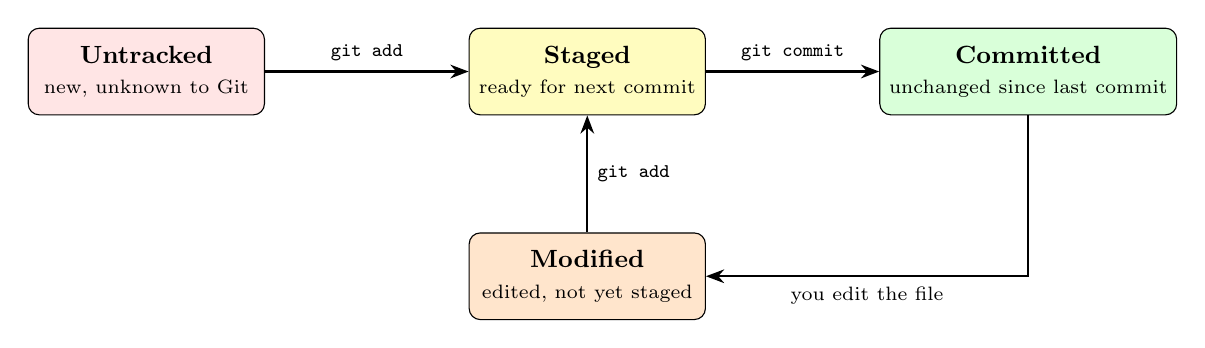
\begin{tikzpicture}[
  st/.style={draw,rounded corners,minimum width=30mm,minimum height=11mm,align=center,font=\small}]
  \node[st,fill=red!10]    (un) at (0,0)    {\textbf{Untracked}\\\scriptsize new, unknown to Git};
  \node[st,fill=yellow!25] (sg) at (5.6,0)  {\textbf{Staged}\\\scriptsize ready for next commit};
  \node[st,fill=green!15]  (cm) at (11.2,0) {\textbf{Committed}\\\scriptsize unchanged since last commit};
  \node[st,fill=orange!20] (md) at (5.6,-2.6) {\textbf{Modified}\\\scriptsize edited, not yet staged};
  \draw[cmdarrow] (un) -- node[above,font=\scriptsize\ttfamily] {git add} (sg);
  \draw[cmdarrow] (sg) -- node[above,font=\scriptsize\ttfamily] {git commit} (cm);
  \draw[cmdarrow] (cm.south) |- node[pos=0.75,below,font=\scriptsize] {you edit the file} (md.east);
  \draw[cmdarrow] (md) -- node[right,font=\scriptsize\ttfamily] {git add} (sg);
\end{tikzpicture}
\caption{States of a file. A file you have never added is \emph{untracked}. After a commit it is \emph{committed}; editing it makes it \emph{modified}; \code{git add} stages it again.}
\label{fig:states}
\end{figure}

A file is \textbf{tracked} if it is in the latest commit or in the staging area; otherwise it is \textbf{untracked}. \code{git status} reports the states in its own words:

\begin{center}
\small
\begin{tabular}{@{}l l@{}}
\toprule
State & What \code{git status} prints \\
\midrule
Untracked & under \code{Untracked files:} \\
Modified & under \code{Changes not staged for commit:}, as \code{modified:} \\
Staged & under \code{Changes to be committed:} \\
Committed & not listed at all (nothing to report) \\
\bottomrule
\end{tabular}
\end{center}

\Needspace{16\baselineskip}
\section{Your first commit, step by step}

We will build a small recipe collection. Make a new folder and a repository, and two files:

\begin{lstlisting}
$ mkdir recipes
$ cd recipes
$ git init
$ echo "# Recipes" > README.md
$ echo "Pancakes: flour, milk, eggs" > recipes.txt
$ git status --short
?? README.md
?? recipes.txt
\end{lstlisting}

\code{git status --short} is a compact form of \code{git status}: one line per file. \code{??} means untracked. (Committing needs the name and email you set in Lecture 1; if Git answers \code{Please tell me who you are}, repeat the \code{git config} step.)

\textbf{Step 1: stage.} Put \code{README.md} in the staging area:

\begin{lstlisting}
$ git add README.md
$ git status
On branch main

No commits yet

Changes to be committed:
  (use "git rm --cached <file>..." to unstage)
	new file:   README.md

Untracked files:
  (use "git add <file>..." to include in what will be committed)
	recipes.txt
\end{lstlisting}

\code{README.md} is now \emph{staged} (``Changes to be committed'') and \code{recipes.txt} is still untracked. We chose to stage only one of the two files. (Git's hints in brackets, such as ``to unstage'', are ways to undo things. We learn them in Lecture 3, so ignore them for now.)

\textbf{Step 2: commit.} Save what is staged, with a message after \code{-m}:

\begin{lstlisting}
$ git commit -m "Add README"
[main (root-commit) ed0e373] Add README
 1 file changed, 1 insertion(+)
 create mode 100644 README.md
$ git status --short
?? recipes.txt
\end{lstlisting}

The first line says: branch \code{main}, this is the \emph{root commit} (the very first, with no parent), its ID is \code{ed0e373}, and its message. \code{recipes.txt} is still untracked because we never staged it, so it is \emph{not} part of this commit.

\Needspace{8\baselineskip}
\textbf{Step 3: the next commit.} Stage and commit the recipes:

\begin{lstlisting}
$ git add recipes.txt
$ git commit -m "Add recipes"
[main 2ee8406] Add recipes
 1 file changed, 1 insertion(+)
 create mode 100644 recipes.txt
\end{lstlisting}

\textbf{Looking at the history.} The command \code{git log --oneline} lists your commits, newest first, one per line, as ID and message:

\begin{lstlisting}
$ git log --oneline
2ee8406 Add recipes
ed0e373 Add README
\end{lstlisting}

These are the first two boxes of Figure~\ref{fig:chain}. (Lecture 3 explores the history in depth. If the output fills the screen and stops, press \code{q} to quit it.)

\begin{quickfact}
On Windows, Git may print a warning such as \code{LF will be replaced by CRLF} when you \code{git add}. It is about line endings, is harmless here, and can be ignored.
\end{quickfact}

\begin{pitfall}
Committing does nothing with a file you never staged. A very common beginner surprise is a missing file in the commit because it was untracked. Run \code{git status} \emph{before} committing and read it.
\end{pitfall}

\subsection{Modified files and selective commits}

Now edit both files. Both are tracked now, so they show as \emph{modified}:

\begin{lstlisting}
$ echo "Crepes: flour, milk, eggs" >> recipes.txt
$ echo "- add more recipes" >> README.md
$ git status
On branch main
Changes not staged for commit:
  (use "git add <file>..." to update what will be committed)
  (use "git restore <file>..." to discard changes in working directory)
	modified:   README.md
	modified:   recipes.txt

no changes added to commit (use "git add" and/or "git commit -a")
$ git status --short
 M README.md
 M recipes.txt
\end{lstlisting}

In the short form each line has \emph{two} columns before the file name: the \textbf{left} column describes the staging area, the \textbf{right} column the working directory. So \code{\ M} (a space, then \code{M}) means ``modified in the working directory, not staged''. Now stage only one file and look again:

\begin{lstlisting}
$ git add recipes.txt
$ git status --short
M  recipes.txt
 M README.md
\end{lstlisting}

\code{M\ \ } (\code{M} in the left column) means ``staged''. \code{recipes.txt} is in the staging area and \code{README.md} is not, so a commit now includes \code{recipes.txt} only. Commit it, then stage and commit the other file as its own commit:

\begin{lstlisting}
$ git commit -m "Add crepes recipe"
$ git add README.md
$ git commit -m "Update README"
$ git status
On branch main
nothing to commit, working tree clean
\end{lstlisting}

\code{working tree clean} means nothing is modified, staged or untracked. This table follows both files through these steps:

\begin{center}
\small
\begin{tabular}{@{}l l l@{}}
\toprule
After this step & \code{README.md} & \code{recipes.txt} \\
\midrule
both edited & modified & modified \\
\code{git add recipes.txt} & modified & \textbf{staged} \\
\code{git commit -m "Add crepes recipe"} & modified & committed \\
\code{git add README.md} & \textbf{staged} & committed \\
\code{git commit -m "Update README"} & committed & committed \\
\bottomrule
\end{tabular}
\end{center}

The same file can even be in two areas at once: if you stage a file and then edit it again, the \emph{staged} version is the earlier one and the later edit is still ``modified''. \code{git status} then lists the file under both headings (\code{MM} in the short form).

\begin{tryit}
Make a new repository, then create and commit two files. Edit both. Stage only one, run \code{git status} and \code{git status --short}, then commit. Which file is left over, and in which state? Then stage and commit the other one, and look at \code{git log --oneline}.
\end{tryit}

\section{Handy variations}

\begin{center}
\small
\begin{tabular}{@{}l >{\raggedright\arraybackslash}p{9.6cm}@{}}
\toprule
Command & Meaning \\
\midrule
\code{git add file1 file2} & Stage several named files. \\
\code{git add .} & Stage \emph{everything} new or changed in the current folder and below. Convenient, but check \code{git status} first so you do not stage what you did not mean to. \\
\code{git commit -m "msg"} & Commit what is staged, with a one-line message. \\
\code{git commit -am "msg"} & Shortcut: stage all changes to files Git already tracks, then commit. It does \emph{not} include untracked (new) files. \\
\bottomrule
\end{tabular}
\end{center}

Deleting files, undoing a staged change and going back to an older version are the subject of Lecture 3.

\section{Writing good commit messages}

The message is for your future self and your teammates. Months later, \code{Fixed stuff} tells nobody anything. A common convention:

\begin{itemize}
  \item A short first line (about 50 characters), written as a command: \emph{Add}, \emph{Fix}, \emph{Remove}, \emph{Update}.
  \item It says \emph{what} the commit does, and, when it matters, why.
  \item No full stop at the end.
\end{itemize}

\Needspace{9\baselineskip}
\begin{center}
\small
\begin{tabular}{@{}p{5.4cm} p{7.4cm}@{}}
\toprule
Weak & Better \\
\midrule
\code{stuff} & \code{Add pancake recipe} \\
\code{fixed it} & \code{Fix typo in README title} \\
\code{update} & \code{Update serving size for crepes} \\
\code{asdf} & \code{Remove unused test file} \\
\bottomrule
\end{tabular}
\end{center}

\begin{pitfall}
If you type \code{git commit} \emph{without} \code{-m}, Git opens a text editor for the message. On many computers the default editor is \code{vim}, which confuses beginners (it does not accept normal typing). To get out without committing, press \code{Esc}, type \code{:q!} and press Enter. To avoid the problem, either always use \code{-m "..."}, or choose an editor you know, for example \code{git config --global core.editor "nano"} (if \code{nano} is available on your computer).
\end{pitfall}

\begin{keyidea}
Make \emph{small, focused} commits: one idea per commit. They are easier to understand, to review, and (in later lectures) to undo.
\end{keyidea}

\Needspace{14\baselineskip}
\section{Ignoring files: \texttt{.gitignore}}

Some files should never be in the history: generated files, temporary logs, large downloads, and above all \emph{secrets} such as passwords. Tell Git to ignore them with a plain text file named \code{.gitignore} in the project folder:

\begin{lstlisting}
# generated and private files
*.log
secret.env
build/
\end{lstlisting}

Each line is a \emph{pattern}:
\begin{itemize}
  \item \code{*.log} ignores every file whose name ends in \code{.log} (\code{*} matches any characters within a name);
  \item \code{secret.env} ignores that exact file;
  \item \code{build/} ignores any folder named \code{build} (the trailing \code{/} means folder);
  \item a line starting with \code{!} is an exception placed \emph{after} the rule it overrides (\code{!keep.log} un-ignores that file);
  \item a line starting with \code{\#} is a comment. Comments must be on their own line.
\end{itemize}

Continue in the clean \code{recipes} repository. Create a log file and the ignore file (the first \code{echo} uses \code{>} to start the file, the others use \code{>>} to append; a text editor works too):

\begin{lstlisting}
$ echo "temporary output" > debug.log
$ echo "# generated and private files" > .gitignore
$ echo "*.log" >> .gitignore
$ echo "secret.env" >> .gitignore
$ echo "build/" >> .gitignore
$ git status --short
?? .gitignore
\end{lstlisting}

\Needspace{9\baselineskip}
\code{debug.log} does not appear: Git ignores it. The \code{.gitignore} file itself is untracked, and \emph{should} be committed so that everyone who clones the project ignores the same things:

\begin{lstlisting}
$ git add .gitignore
$ git commit -m "Add .gitignore"
\end{lstlisting}

Your history now has five commits, and \code{git log --oneline} shows them all.

\begin{pitfall}
\textbf{Ignoring only affects files that are not yet tracked.} If you already committed a file, adding it to \code{.gitignore} does not remove it from the project or from the history. (Lecture 3 shows how to stop tracking a file.)
\end{pitfall}

\begin{pitfall}
\textbf{Never commit passwords, keys or tokens.} Git remembers every commit, so deleting the file later does \emph{not} erase it from history. If a secret is ever committed, treat it as leaked: change the password or revoke the key. Put such files in \code{.gitignore} \emph{before} the first \code{git add}.
\end{pitfall}

\Needspace{36\baselineskip}
\section{Homework 2}

\begin{homework}{2: Snapshots}
From the course folder (\code{LearningGit/}) run:
\begin{lstlisting}
$ bash codeHints/L02/setup_hw2.sh
$ cd practice/hw2
\end{lstlisting}
The setup script creates a repository \code{practice/hw2} (with a local identity already set) containing five files and a folder, and \textbf{no commits}: \code{README.md}, \code{notes.txt}, \code{todo.txt}, \code{debug.log}, \code{secret.env}, and the folder \code{build/} (which contains one file, \code{output.bin}). Run \code{git status} to look. Then do the tasks \emph{in this order}:

\begin{description}[leftmargin=1.2em,style=nextline]
\item[2.1 First commit] Commit \code{README.md} and \code{notes.txt} \emph{only}, with the message \code{Add README and notes}.
\item[2.2 Second commit] Commit \code{todo.txt} with the message \code{Add todo list}.
\item[2.3 Ignore] Create a \code{.gitignore} so that \code{debug.log}, \code{secret.env} and the \code{build/} folder are ignored. Commit it with the message \code{Add .gitignore}. After this, \code{git status} must not list the three ignored items, and \code{git log --oneline} shows three commits.
\item[2.4 Two areas at once] Append one new line to \code{notes.txt} and one new line to \code{todo.txt} (use \code{echo "..." >> file}). Stage \code{notes.txt} \emph{only}, and do \textbf{not} commit (the checker expects the changes to be uncommitted). Then \code{git status --short} must show exactly two lines: \code{M\ \ notes.txt} (staged) and \code{\ M todo.txt} (modified, not staged).
\item[2.5 Question] Outside the repository, in the file \code{practice/hw2\_areas.txt}, write the name of the area that \code{git add} copies changes into.
\end{description}

\textbf{Check yourself:} from the course folder, \code{bash codeHints/L02/check\_hw2.sh}. All \code{PASS}, then compare with the solutions at the end of this lecture (or in \code{solutions/L02/}).
\end{homework}

\section{Summary}

\begin{itemize}
  \item A commit is a snapshot of the whole project plus a message, author and date. History is a chain of commits, each pointing to its parent.
  \item Three areas: working directory $\to$ (\code{git add}) staging area $\to$ (\code{git commit}) repository.
  \item Files are untracked, modified, staged or committed; \code{git status} tells you which.
  \item Stage only what belongs together; write short, imperative messages.
  \item \code{.gitignore} keeps unwanted files out. Never commit secrets.
\end{itemize}

\textbf{Further reading:} \emph{Pro Git} (\url{https://git-scm.com/book}), Chapter 2.2 ``Recording Changes to the Repository'' (it also covers \code{.gitignore}); manual pages \code{git help add}, \code{commit}, \code{gitignore}.

\solutionspage

\section*{Solutions to Homework 2}

Run from the course folder, then work inside \code{practice/hw2}:

\begin{lstlisting}
$ bash codeHints/L02/setup_hw2.sh
$ cd practice/hw2
$ git add README.md notes.txt
$ git commit -m "Add README and notes"
$ git add todo.txt
$ git commit -m "Add todo list"
$ echo "debug.log" > .gitignore
$ echo "secret.env" >> .gitignore
$ echo "build/" >> .gitignore
$ git add .gitignore
$ git commit -m "Add .gitignore"
$ echo "Second note." >> notes.txt
$ echo "- practice commits" >> todo.txt
$ git add notes.txt
$ git status --short
M  notes.txt
 M todo.txt
$ echo "staging area" > ../hw2_areas.txt
\end{lstlisting}

\textbf{2.1.} Staging only the two named files leaves \code{todo.txt} untracked, so it is not in the first commit. \code{git add .} here would have wrongly included \code{todo.txt}, \code{debug.log}, \code{secret.env} and \code{build/}. If you made a mistake before committing, \code{git status} shows what is staged; you will learn to unstage in Lecture 3.

\textbf{2.2.} Commit \code{todo.txt} on its own, so the history reads naturally.

\textbf{2.3.} Create the ignore file \emph{before} anything adds the secrets. Check that \code{git status} no longer mentions the three items. (Optional: \code{git check-ignore -v debug.log secret.env build/output.bin} prints which rule matched each file.) \code{*.log} instead of \code{debug.log} also passes the checker.

\textbf{2.4.} The \emph{first} column of \code{git status --short} describes the staging area, the \emph{second} the working directory. \code{M\ \ notes.txt} means ``staged change''; \code{\ M todo.txt} means ``modified but not staged''. A commit now would include only \code{notes.txt}. (Do not commit: the checker expects this state.)

\textbf{2.5.} The \textbf{staging area}, also called the \textbf{index}. The answer file sits in \code{practice/}, outside \code{hw2}, so that it does not appear as an untracked file in the repository.

\Needspace{8\baselineskip}
\textbf{Common mistakes.}
\begin{itemize}
  \item Using \code{git add .} too early, which stages \code{secret.env} and the build files. Look at \code{git status} first.
  \item Wrong commit messages: the checker compares them exactly, including capital letters.
  \item Committing in task 2.4. If you did, the checker will report four commits. You can run \code{setup\_hw2.sh --reset} and do the tasks again.
  \item Forgetting \code{-m}: an editor opens. Press \code{Esc}, type \code{:q!}, press Enter, and try again.
\end{itemize}


\end{document}
